En este capítulo se presentan los objetivos que se buscan alcanzar al concluir la implementación del sistema y los puntos que se desean cubrir para resolver la problemática anteriormente presentada, se 
explica la arquitectura del sistema, la forma de trabajo que se utilizará durante el desarrollo del sistema, el flujo del negocio, así como los requerimientos del mismo.\\
\newline

Recordemos que las plataformas de bolsa de trabajo universitarias al ser diseñadas únicamente para su comunidad estudiantil no se puede acceder 
a su información tan fácilmente y están diseñadas para satisfacer sus objetivos y necesidades de la propia universidad y comunidad por lo que los objetivos y las necesidades que debe de cubrir una bolsa de trabajo para la ESCOM o  el IPN en general son diferentes en comparación con el Tecnológico de Monterrey o de la Universidad Autónoma de México.\\
\newline
Antes de poder definir de forma adecuada los requerimientos y el alcance del proyecto se listan las bolsas de trabajo más populares entre las personas que más se apegan al objetivo del Trabajo Terminal, así como  la bolsa de trabajo oficial del Instituto:
\begin{itemize}
    \item OCCMundial
    \item CompuTrabajo
    \item Indeed
    \item Siboltra 
    \item ESCOMobile: a pesar de que esta aplicación no es una bolsa de trabajo, en ella se pueden consultar los boletines de trabajo
    publicados por la ESCOM.
\end{itemize}
En la tabla \ref{table:herramientasSimilares} se muestran las características de cada una de ellas y las características que pretende tener el Trabajo Terminal.
%\newpage


\begin{longtable}{| p{0.15\textwidth}  | p{0.10\textwidth} | p{0.10\textwidth}  | p{0.10\textwidth}  | p{0.10\textwidth}  | p{0.10\textwidth}  |  p{0.10\textwidth}  |}

    \hline

    \textbf{Herramienta} & \IUocc{}	& \IUcompuT{}&  \IUIneed{} & \IUsisae{} & \scriptsize \textbf{ESCOMobile} & \scriptsize Trabajo Terminal\\ 
    \hline

    Contacto directo reclutador-candidato dentro de la plataforma & Sí & No  & Sí  & No  & No & Si.\\ \hline
    Filtrado automático de currículos recibidos & Sí & Sí & No & No & No & Si.\\ \hline
    Autogenerado de CV & Sí & Sí & Sí  & No & Sí & Sí. \\ \hline
    Seguimiento del estado de solicitud & Sí  & Sí & No & No  & Si& Sí. \\ \hline
    Búsqueda de candidatos & Sí & Sí & Sí & Sí & No & Sí\\ \hline

    \caption{Comparación Plataformas para buscar empleo}
    \label{table:herramientasSimilares}
\end{longtable}

En general todas las plataformas cumplen con publicar vacantes y consultar perfiles de candidatos, pero el publicar una vacante y dejarla visible en la plataforma para que se postulen no siempre es gratuito, la OCCMundial, CompuTrabajo e Indeed cobran por vacante publicada y el tiempo que dure dicha vacante abierta, así como los servicios que te gustaria tener. Si quieres que se te recomienden candidatos cada cierto tiempo tiene un precio extra.\\

En Ineed si quieres que tu vacante publicada tenga cierto patrocinio es decir, que sean de las primeras en ser vistas se te cobra una comisión extra.\\
\newline
Nuestro sistema no se pedirá ninguna comisión por su uso (por el simple hecho que es que para la comunidad de ESCOM), tampoco tendrá límite de vacantes publicadas, el reclutador tendrá total libertad en consultar candidatos y configurar la fecha de publicación y cierre sus vacantes. \\

Un punto importante es que resolverá los problemas de gestión de vacantes  y correos para validar la información de las empresas que actualmente tiene el departamento de extensión y apoyos educativos de la ESCOM.\\
\newline
Con base en lo anterior se redacta el objetivo del proyecto, arquitectura y flujo del sistema.

\section{Objetivo}
\subsection{Objetivo general}
\begin{itemize}
    \item Implementar un sistema web para la Bolsa de trabajo ESCOM, mejorando la búsqueda de vacantes y pueda 
    ofrecer apoyo al proceso de reclutamiento para las empresas con el fin de resolver los problemas de gestión 
    identificados.
\end{itemize}

\subsection{Objetivos específicos}
        \begin{itemize}
            \item Desarrollar una plataforma web para la bolsa de trabajo ESCOM, independiente de la página de Facebook.
            \item Diseñar un procedimiento para el registro de empresas al sistema con base al sistema manejado a la actual 
            implementación de la bolsa de trabajo ESCOM.
            \item Facilitar la publicación de vacantes para los reclutadores, implementando la capacidad de realizar la
            publicación directamente por ellos.
            \item Implementar un algoritmo de clasificación que automatice la búsqueda de los mejores postulantes, analizando su 
            currículum acorde a sus intereses y los intereses de la empresa.
        \end{itemize}
%        \section{Objetivo}
\clearpage
\section{Arquitectura}
En la figura \ref{fig:arquitectura} se muestra el diagrama de la arquitectura del sistema así como sus componentes.
Posteriormente se encuentra la descripción de cada componente del diagrama.

\begin{figure}[hbtp!]
    \begin{center}
        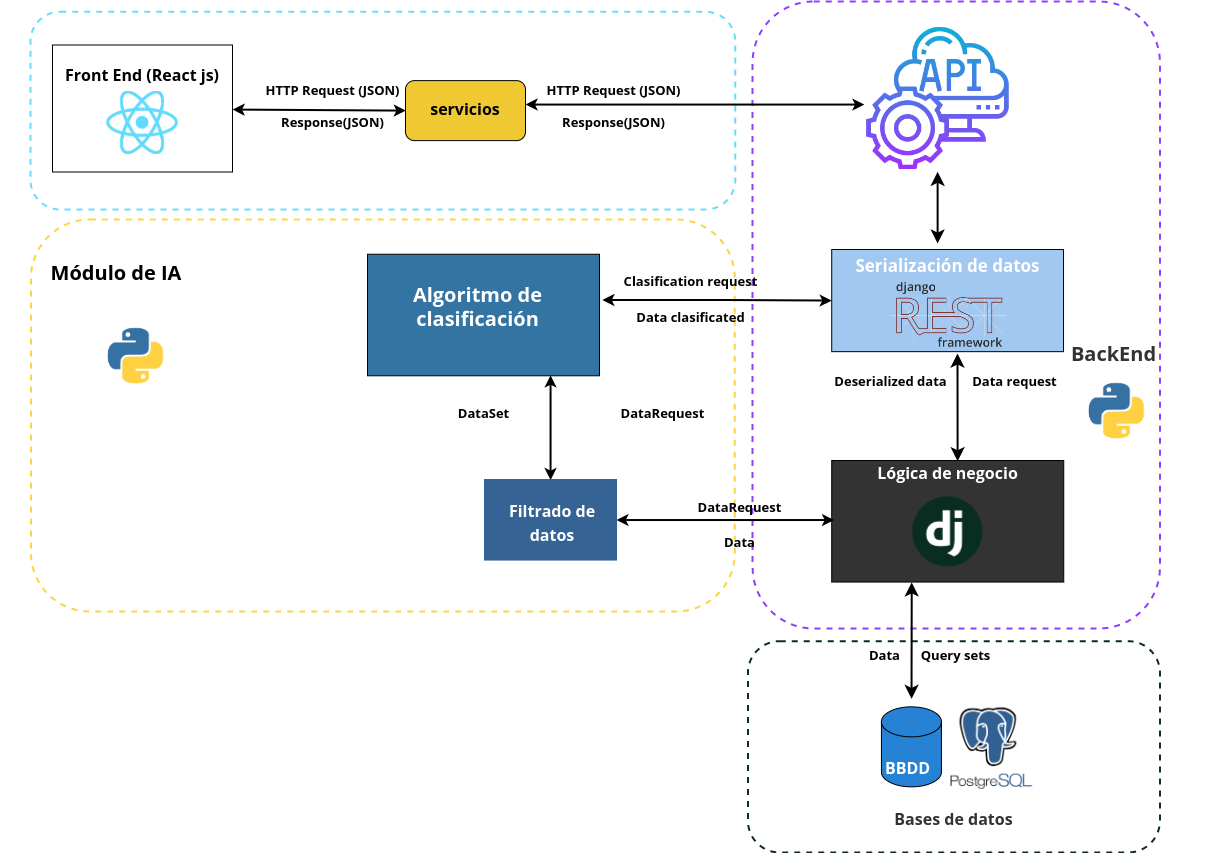
\includegraphics[width=.9\textwidth]{propuesta/imagenes/arqui.png}
    \end{center}
    \caption{Arquitectura del sistema}
    \label{fig:arquitectura}
\end{figure}


%\begin{description}
%    \item[Servidor Web] El servidor web es el punto de entrada a nuestra herramienta, en el se alberga el código HTML, 
%    CSS y JS compilado React Js.
    %\item[Bases de Datos] Cada servicio de nuestra arquitectura cuenta con su propia base de datos. Esto es para eliminar la dependencia entre ellos. Todas las bases de datos utilizan el gestor de Postgres debido a su eficiencia en desempeño y consultas además de que es open source.
%\end{description}
\clearpage
\section{Flujo del sistema}
En esta sección vamos a describir de forma general el flujo que se debe seguir cualquier usuario cuando interactué con el sistema y que se puede ver en la figura .
\begin{figure}[H]
    \begin{center}
        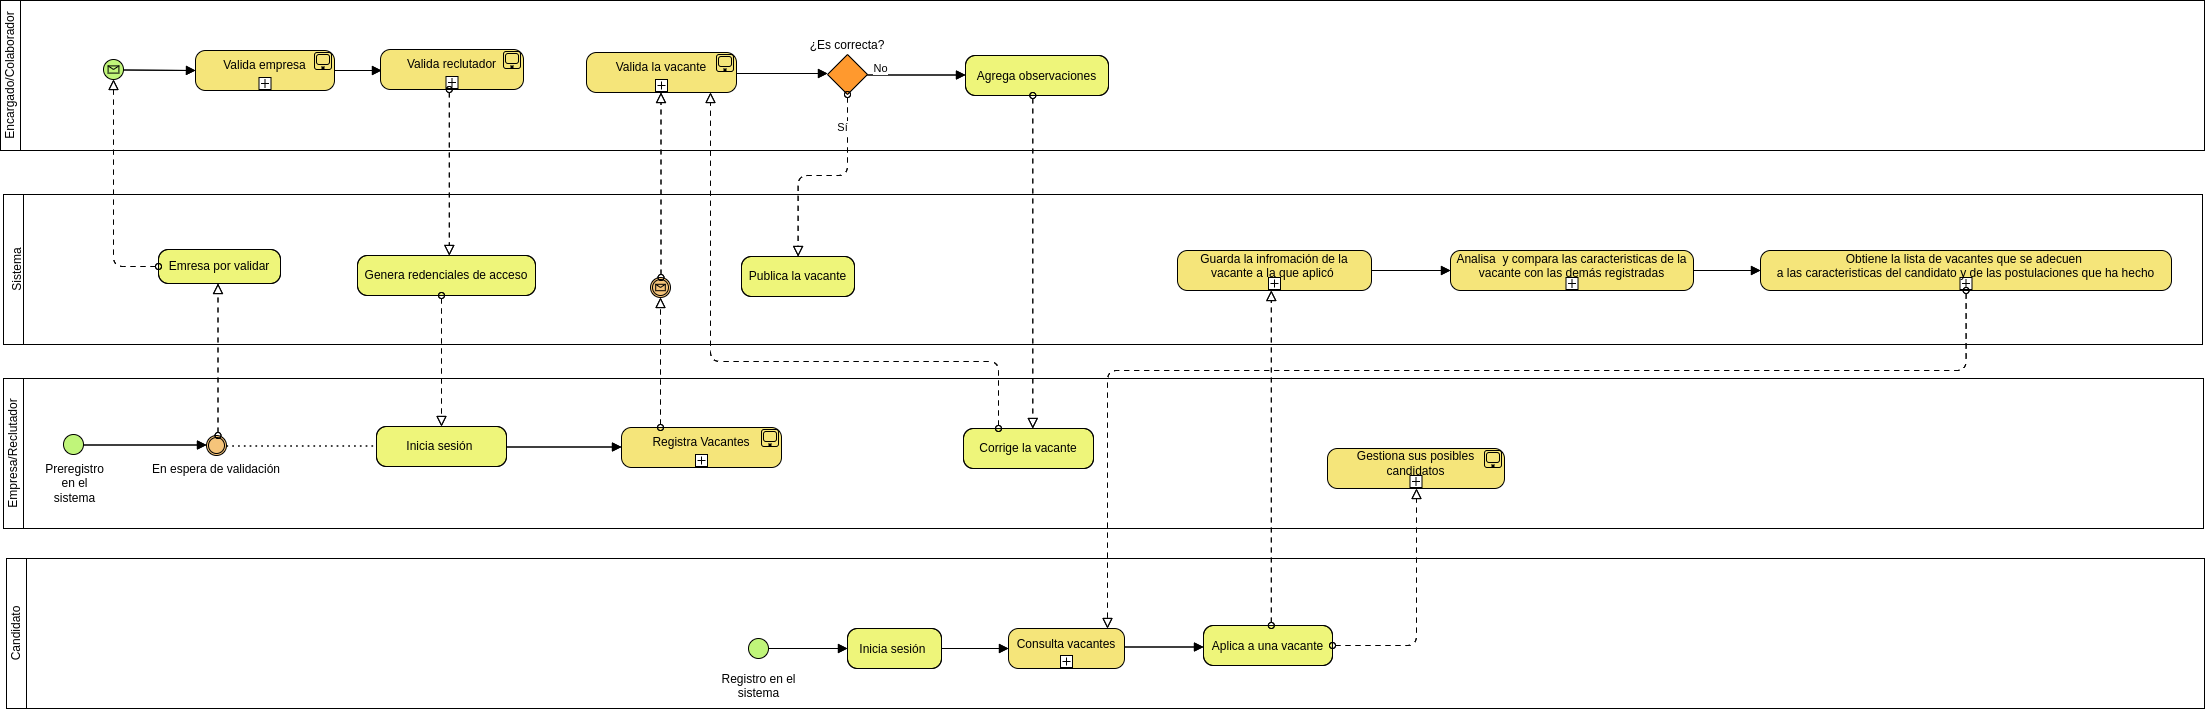
\includegraphics[height=0.27\textheight,angle=90]{propuesta/imagenes/Flujo.png}
    \end{center}
    \caption{Flujo del sistema.}
    \label{mark:top}
\end{figure}


Por negocio se identificaron 4 usuarios que pueden interactuar con el sistema:
\begin{itemize}
    \item \refElem{aCandidato}
    \item \refElem{aReclutador}
    \item \refElem{aColaborador}
    \item \refElem{aEncargado}
\end{itemize} 

DIchos actores estarán participando en 4 procesos importantes del sistema, a continuación se describen de manera breve dichos procesos:
\begin{itemize}
    \item Gestión de usuarios: en esta etapa se registran y validan reclutadores y empresas y si es necesario el encargado del sistema puede registrar más colaboradores dentro del sistema.\\Se puede tener más de un reclutador por empresa siempre y cuando sea validado por en encargado o colaborador del sistema.\\Solo existe un encargado en el sistema y solo el podrá registrar más colaboradores.
    \item Gestión de vacantes: en este proceso los reclutadores que hayan sido validados por el encargado y/o el mismo encargado del sistema podrán registrar vacantes. Sí el reclutador registra una vacante, esta tiene que ser validada por el encargado o colaborador del sistema, en dado caso que el colaborador encuentre detalles en la vacante podrá enviar observaciones al reclutador que haya creado la vacante y en consecuencia el reclutador la podrá corregir las veces que sean necesarias hasta que el encargado/colaborador le de visto bueno. Una vacante aprobada por el encargado/colaborador será publicada inmediatamente en el sistema. 
    \item Gestión de postulaciones: en este proceso los reclutadores podrán consultar loas perfiles de los candidatos que se hayan postulado a sus vacantes publicadas, asi como los candidatos recomendados para decidir quien continua con el proceso de postulación para la oferta o quien es descartado del proceso.% cabe recalcar que por cuestiones de privacidad y de negocio el reclutador solo podrá consultar los perfiles de l
    \item Recomendación de vacantes/candidatos: esta etapa es interna del sistema, cada vez que un candidato se postula a una vacante el sistema guarda la información de dichas postulaciones que el candidato haya hecho. Dichos datos son almacenados y comparados para hacer el proceso de recomendación tomando en cuenta dos factores:
    \begin{itemize}
        \item Las características del candidato que tiene registradas en su perfil y las de las vacantes que hay en el sistema registradas.
        \item Las características de las vacantes que el candidato se haya postulado y las de las vacantes que hay en el sistema registradas.
    \end{itemize} 
\end{itemize} 

\clearpage
\section{Planeación del proyecto}
Para el desarrollo de este proyecto se escogió la metodología SCRUM, el cual está enfocada a la
entrega periódica de resultados que agreguen valor al proyecto, además en esta metodología todos los integrantes del
equipo conocen el que ocurre y cuando en el proyecto, haciendo la comunicación más eficiente en caso de que se presenten errores
o se necesiten realizar cambios en la implementación.\\
Las fases de la metodología son iterativas y el ciclo se repite cada determinado tiempo, a esto se le llama
sprint y se compone de 3 fases:

 \begin{itemize}
    \item \textbf{Planeación del Sprint}: En esta fase se realiza una junta para planear los objetivos del sprint y las a actividades
    a realizar para lograrlos.
    \item \textbf{Ejecución del Sprint}: En esta fase ser realizan las actividades planeadas y se realizan juntas diarias de máximo
    15 minutos donde se exponen las actividades realizadas, las actividades que se están realizando y los
    impedimentos para completar las actividades.
    \item \textbf{Revisión del Sprint}: En esta fase se entregan los resultados obtenidos durante el sprint y se revisan los errores
    y retrasos ocurridos durante el sprint.
 \end{itemize}



Se seleccionó SCRUM por sus características para desarrollar proyectos que facilitara el proceso de diseñar e
implementar el proyecto con la menor cantidad de errores posibles.\\

Las actividades y roles que vamos a adoptar de Scrum son los siguientes:
\begin{itemize}
    \item \textbf{El equipo de Scrum}: Compuesto por un Scrum Master y el Development Team. En el caso de este trabajo el
rol de Scrum Master va a ser tomado por ambos directores y el rol Development Team va a ser tomado por
nosotros que presnetaremos el trabajo terminal.
    \item \textbf{El sprint}: Como ya anteriormente se explicó en que consiste, para este proyecto se manejaran sprints de 15
días. Al final de cada sprint se deben entregar resultados para ajustar las estrategias y comenzar el siguiente
sprint.
    \item \textbf{Product Backlog}: Es el listado de tareas que engloba todo un proyecto. Cualquier cosa que debamos hacer
debe estar en el product backlog y con un tiempo estimado por el equipo de desarrollo.
\end{itemize}


El total de interaciones o sprints que tendrá el sistema será de 18 sprints separados a nivel de dependencias es decir, el primero
completará los objetivos del segundo y asi sucesivamente de tal manera que el sprint que este en ejecución 
no necesite del siguiente que se vaya ejecutar.
\newline

En la figura \ref{fig:cronograma} se muestra el diagrama de Gantt en el que se puede apreciar los sprits del desarrollo del sistema.La
Posteriormente se encuentra la descripción de cada componente del diagrama.

\begin{figure}[hbtp!]
    \begin{center}
        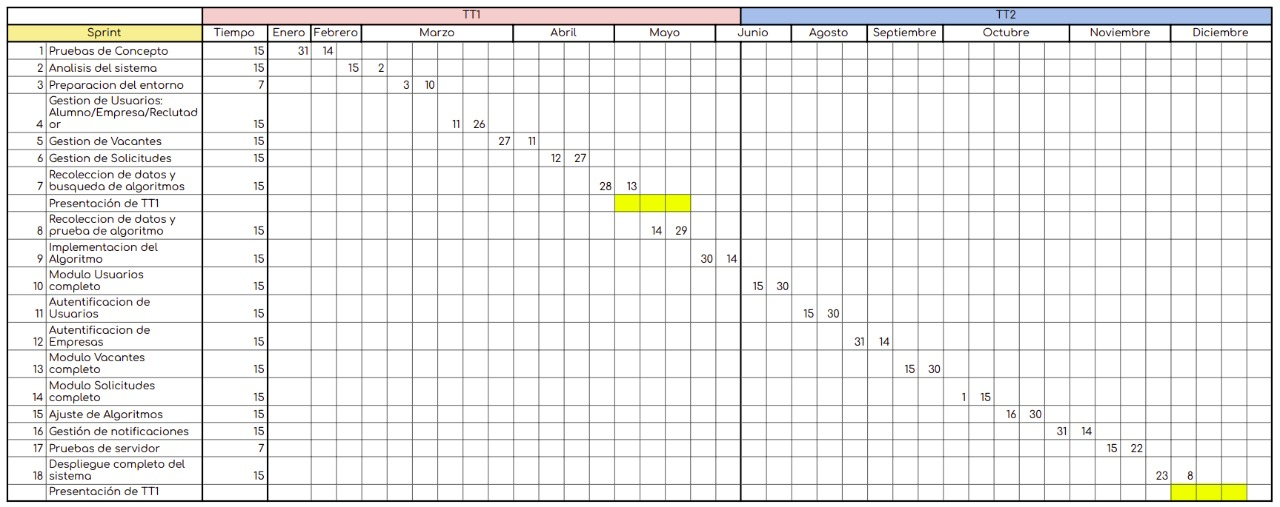
\includegraphics[width=1\textwidth]{propuesta/imagenes/gantt.jpeg}
    \end{center}
    \caption{Diagrama de Gantt del sistema}
    \label{fig:cronograma}
\end{figure}

En la entrega de TT1 los sprints que se van a ejecutar son:

\begin{itemize}
    \item \textbf{Sprint 1}: Pruebas de Concepto.
    \item \textbf{Sprint 2}: Analisis del sistema.
    \item \textbf{Sprint 3}: Preparacion del entorno.
    \item \textbf{Sprint 4}: Gestion de Usuarios: Alumno/Empresa/Reclutador.
    \item \textbf{Sprint 5}: Gestion de Vacantes.
    \item \textbf{Sprint 6}: Gestion de Solicitudes.
    \item \textbf{Sprint 7}: Recoleccion de datos y busqueda de algoritmos.
\end{itemize}


En la entrega de TT2 los sprints que se van a ejecutar son:

\begin{itemize}
    \item \textbf{Sprint 8}:  Recoleccion de datos y prueba de algoritmo.
    \item \textbf{Sprint 9}:  Implementacion del Algoritmo.
    \item \textbf{Sprint 10}: Modulo Usuarios completo.
    \item \textbf{Sprint 11}: Autentificacion de Usuarios. 
    \item \textbf{Sprint 12}: Autentificacion de Empresas.
    \item \textbf{Sprint 13}: Modulo Vacantes completo.
    \item \textbf{Sprint 14}: Modulo Solicitudes completo.
    \item \textbf{Sprint 15}: Ajuste de Algoritmos.
    \item \textbf{Sprint 16}: Gestión de notificaciones.
    \item \textbf{Sprint 17}: Pruebas de servidor.
    \item \textbf{Sprint 18}: Despliegue completo del sistema.
\end{itemize}


%\section{Arquitectura}

